%!TEX TS-program = xelatex

% Шаблон документа LaTeX создан в 2018 году
% Алексеем Подчезерцевым
% В качестве исходных использованы шаблоны
% 	Данилом Фёдоровых (danil@fedorovykh.ru) 
%		https://www.writelatex.com/coursera/latex/5.2.2
%	LaTeX-шаблон для русской кандидатской диссертации и её автореферата.
%		https://github.com/AndreyAkinshin/Russian-Phd-LaTeX-Dissertation-Template

\documentclass[a4paper,14pt]{article}

\input{data/preambular.tex}
\begin{document} % конец преамбулы, начало документа
\begin{titlepage}
	\begin{center}
		ФЕДЕРАЛЬНОЕ  ГОСУДАРСТВЕННОЕ АВТОНОМНОЕ \\
		ОБРАЗОВАТЕЛЬНОЕ УЧРЕЖДЕНИЕ ВЫСШЕГО ОБРАЗОВАНИЯ\\
		«НАЦИОНАЛЬНЫЙ ИССЛЕДОВАТЕЛЬСКИЙ УНИВЕРСИТЕТ\\
		«ВЫСШАЯ ШКОЛА ЭКОНОМИКИ»
	\end{center}
	
	\begin{center}
		\textbf{Московский институт электроники и математики}
		
		\textbf{Им. А.Н.Тихонова НИУ ВШЭ}
		
		\textbf{Департамент компьютерной инженерии}
	\end{center}
	\vspace{1ex}	
	\begin{center}
		Подчезерцев Алексей Евгеньевич, группа БИВ174
		
		Солодянкин Андрей Александрович, группа БИВ174
	\end{center}	
	\vspace{1ex}
	\begin{center}
		\textbf{ОТЧЕТ\\
		ПО ЛАБОРАТОРНОЙ РАБОТЕ №1
	}
	\end{center}	
	\vspace{2ex}
	\begin{center}
		по дисциплине «Проектирование систем на кристалле»
	\end{center}

	\vfill
	\begin{center}
		Москва \the\year \, г.
	\end{center}
\end{titlepage}
\tableofcontents
\pagebreak

\section{Задание}

Исходная таблица истинности.

\begin{table}[H]
	\caption{Таблица истинности}
	\centering
	\begin{tabular}{|c|c|c|c?{2pt}c|}
		\hline
	$x_1$ & $x_2$ & $x_3$ & $x_4$ & $y$ \\ \hline
	0     & 0     & 0     & 0     & 0   \\ \hline
	0     & 0     & 0     & 1     & 1   \\ \hline
	0     & 0     & 1     & 0     & 0   \\ \hline
	0     & 0     & 1     & 1     & 1   \\ \hline
	0     & 1     & 0     & 0     & 1   \\ \hline
	0     & 1     & 0     & 1     & 0   \\ \hline
	0     & 1     & 1     & 0     & 1   \\ \hline
	0     & 1     & 1     & 1     & 1   \\ \hline
	1     & 0     & 0     & 0     & 0   \\ \hline
	1     & 0     & 0     & 1     & 1   \\ \hline
	1     & 0     & 1     & 0     & 1   \\ \hline
	1     & 0     & 1     & 1     & 1   \\ \hline
	1     & 1     & 0     & 0     & 0   \\ \hline
	1     & 1     & 0     & 1     & 1   \\ \hline
	1     & 1     & 1     & 0     & 0   \\ \hline
	1     & 1     & 1     & 1     & 1   \\ \hline
	\end{tabular}
\end{table}

\section{Выполнение работы}

Постоим данную схему в графическом редакторе Quartus Prime Lite Edition. 
Сделаем несколько реализаций -- СКНФ, СДНФ, минимизированную схему.
Части схем представлены на рис. \ref{fig:schema_01} - \ref{fig:schema_03}.

\begin{figure}[H]
	\centering
	\includegraphics[width=0.8\linewidth]{image/schema_01}
	\caption{СКНФ для представленного выражения}
	\label{fig:schema_01}
\end{figure}

\begin{figure}[H]
	\centering
	\includegraphics[width=0.8\linewidth]{image/schema_02}
	\caption{СДНФ для представленного выражения}
	\label{fig:schema_02}
\end{figure}

\begin{figure}[H]
	\centering
	\includegraphics[width=0.8\linewidth]{image/schema_03}
	\caption{Минимизированная СКНФ для представленного выражения}
	\label{fig:schema_03}
\end{figure}

Для реализации данных схем в исходном виде потребуется 16, 11 и 9 логических элементов соответственно.
Посмотрим реальные значения после сборки схемы в программе Quartus Prime Lite Edition (рис. \ref{fig:compilation_report} и \ref{fig:tmv}).


\begin{figure}[H]
	\centering
	\includegraphics[width=0.8\linewidth]{image/compilation_report}
	\caption{Результат компиляции схемы}
	\label{fig:compilation_report}
\end{figure}

\begin{figure}[H]
	\centering
	\includegraphics[width=0.8\linewidth]{image/tmv}
	\caption{TMV представление схемы}
	\label{fig:tmv}
\end{figure}

Как можно заметить, компилятор в каждом случае оптимизировал схему до 2 логических элементов, а в случае реализации всех схем в одном выражении, компилятор объединял все выражения в одно и подавал на различные выходы один и тот же результат. 
Это говорит, с одной стороны, о правильной реализации каждого отдельного варианта схемы, так и о том, что нет в данном случае разницы о способе составления схемы -- компилятор сам оптимизирует схему до такой степени, сколько это возможно.

Посчитаем временные задержки для данной схемы (рис. \ref{fig:time}).

\begin{figure}[H]
	\centering
	\includegraphics[width=0.8\linewidth]{image/time}
	\caption{Задержки для выражения}
	\label{fig:time}
\end{figure}

Как можно заметить, результаты не сильно отличаются друг от друга.

На рис. \ref{fig:wave} изображена waveform для данного выражения.
Можно убедиться в правильности работы схемы.

\begin{figure}[H]
	\centering
	\includegraphics[width=0.8\linewidth]{image/wave}
	\caption{Waveform для схемы}
	\label{fig:wave}
\end{figure}


На рис. \ref{fig:real} изображена ситуация, когда на вход схемы подано значение $1001$, а на каждом из выходов получен высокий активный сигнал.

\begin{figure}[H]
	\centering
	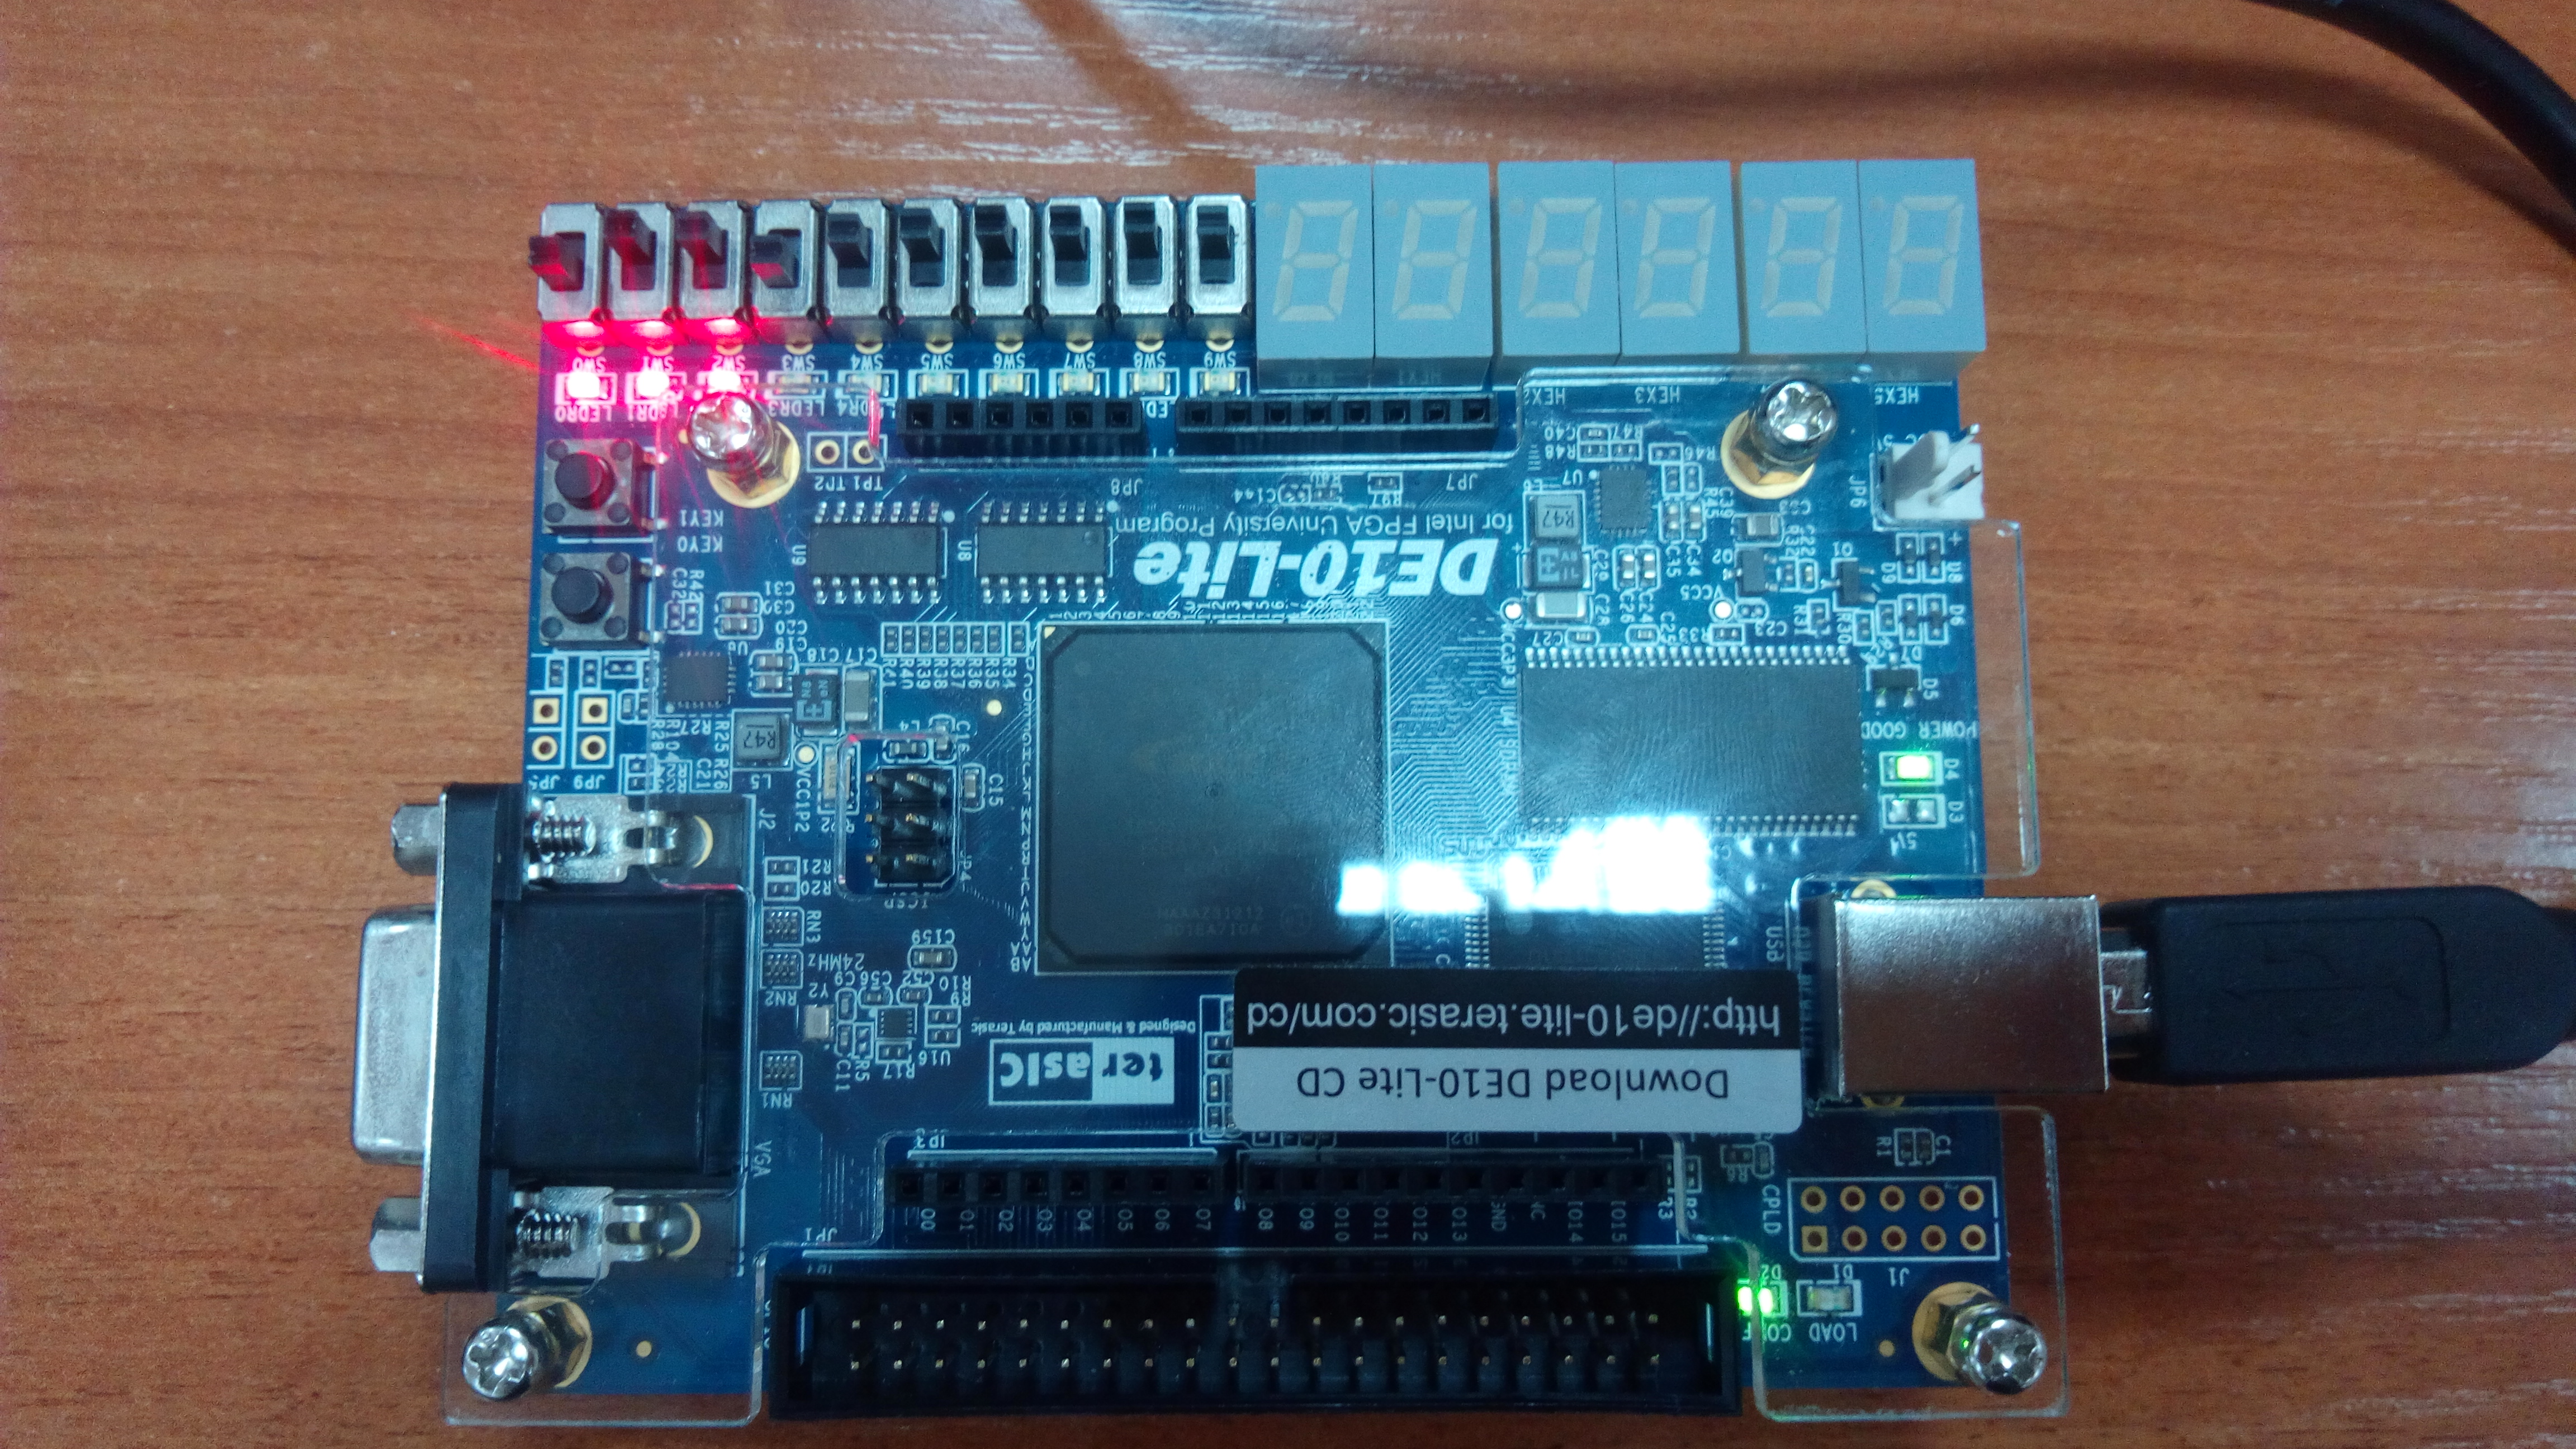
\includegraphics[width=0.8\linewidth]{image/real}
	\caption{Результат работы на плате}
	\label{fig:real}
\end{figure}


\section{Выводы по работе}

В ходе работы были получены выражения в формате СКНФ и СДНФ и в минимизированном варианте, получены результаты моделирования с оптимизацией схемы, рассчитаны временные задержки в с помощью Time Quest Timing Analyzer.
Выяснилось, что итоговая схема не зависит от уровня ручной оптимизации схемы, и что даже разные варианты компилятор приводит к единому виду.
Итоговый вариант был проверен на плате DE10-Lite, наблюдения подтвердили работоспособность устройства и правильность оптимизаций.

\newpage 
\renewcommand{\refname}{{\normalsize Список использованных источников}} 
\centering 
\begin{thebibliography}{9} 
	\addcontentsline{toc}{section}{\refname} 
	\bibitem{Verilog} Thomas D., Moorby P. The Verilog Hardware Description Language. – Springer Science \& Business Media, 2008.
	\bibitem{Quartus} Антонов А., Филиппов А., Золотухо Р. Средства системной отладки САПР Quartus II //Компоненты и технологии. – 2008. – №. 89.
\end{thebibliography}

\end{document} % конец документа